\documentclass{article}
\usepackage[utf8]{inputenc} % Добавляем поддержку UTF-8
\usepackage[T2A]{fontenc}   % Используем кодировку T2A для кириллицы
\usepackage[russian]{babel} % Поддержка русского языка
\usepackage{amsmath, amssymb}
\usepackage{graphicx}
\usepackage{hyperref}
\usepackage{listings}
\usepackage{listingsutf8} % Поддержка UTF-8 для пакета listings
\usepackage{xcolor}
\usepackage{geometry}
\usepackage{float}

\geometry{top=2.5cm, bottom=2.5cm, left=2.3cm, right=2.4cm}

\title{Визуализация фракталов: Множества Мандельброта, Жюлиа и Бассейны Ньютона}
\author{}
\date{}

\begin{document}
	
	\maketitle
	\newpage
	\tableofcontents
	\newpage
	
	\section{Введение}
	В этой лабораторной работе мы исследуем и визуализируем фрактальные множества: множество Мандельброта, множества Жюлиа и бассейны Ньютона. Мы изучим их математические свойства, реализуем алгоритмы для генерации их визуальных представлений и проанализируем полученные результаты.
	
	\section{Определения}
	
	\subsection{Множество Мандельброта}
	\textbf{Определение:} Множество Мандельброта определяется как множество комплексных чисел $c$, для которых последовательность, заданная уравнением
	\begin{equation}
		z_{n+1} = z_n^2 + c, \quad z_0 = 0,
	\end{equation}
	остаётся ограниченной при $n \to \infty$. Иными словами, если величина $|z_n|$ не стремится к бесконечности для данного $c$, то $c$ является частью множества Мандельброта.
	
	\subsection{Множество Жюлиа}
	\textbf{Определение:} Для заданного комплексного параметра $c$ множество Жюлиа $J_c$ — это множество всех точек $z_0$ на комплексной плоскости, для которых последовательность
	\begin{equation}
		z_{n+1} = z_n^2 + c,
	\end{equation}
	начиная с $z_0$, остаётся ограниченной. Множество Жюлиа можно рассматривать как границу между точками, которые приводят к ограниченным и неограниченным последовательностям при итерации функции.
	
	\section{Математические концепции}
	
	\subsection{Итерация и композиция}
	\textbf{Итерация функции:} Обозначение $f^n(z)$ представляет собой $n$-кратную итерацию функции $f$, то есть повторное применение функции $f$ к её результату:
	\begin{equation}
		f^n(z) = \underbrace{f \circ f \circ \cdots \circ f}_{n\ \text{раз}}(z).
	\end{equation}
	Здесь символ $\circ$ обозначает композицию функций, а именно $f \circ g(z) = f(g(z))$.
	
	\subsection{Устойчивость итераций}
	\textbf{Устойчивость итераций:} Итерации функции $f$ считаются устойчивыми в точке $z_0$, если небольшие изменения в начальном значении $z_0$ не приводят к значительным изменениям в последовательности $f^n(z_0)$. Математически это выражается следующим образом:
	\begin{equation}
		\forall\, \varepsilon > 0\ \exists\, \delta > 0:\ \forall\, z,\ |z - z_0| < \delta \implies |f^n(z) - f^n(z_0)| < \varepsilon,\ \forall\, n \in \mathbb{N}.
	\end{equation}
	Это означает, что траектории итераций точек, близких к $z_0$, остаются близкими на всех шагах итерации.
	
	\newpage
	
	\section{Доказательства свойств множества Мандельброта}
	
	\subsection{Доказательство симметрии относительно вещественной оси}
	\textbf{Свойство 1:} Множество Мандельброта симметрично относительно вещественной оси, то есть если $c$ принадлежит множеству, то и его комплексно-сопряжённое $\overline{c}$ также принадлежит множеству.
	
	\textbf{Доказательство:}
	Рассмотрим последовательность:
	\begin{equation}
		z_{n+1} = z_n^2 + c, \quad z_0 = 0.
	\end{equation}
	Пусть для некоторого $c$ последовательность $\{z_n\}$ ограничена. Рассмотрим комплексно-сопряжённое число $\overline{c}$ и соответствующую последовательность $\{\overline{z}_n\}$. Покажем, что она также ограничена.
	
	Используем свойство комплексного сопряжения:
	\begin{equation}
		\overline{z_{n+1}} = \overline{z_n^2 + c} = \overline{z_n}^2 + \overline{c}.
	\end{equation}
	Это означает, что последовательность для $\overline{c}$ является комплексно-сопряжённой к последовательности для $c$. Поскольку модуль комплексно-сопряжённого числа равен модулю исходного числа, то $|\overline{z}_n| = |z_n|$. Таким образом, если последовательность $\{z_n\}$ ограничена, то и $\{\overline{z}_n\}$ ограничена.
	
	Следовательно, если $c$ принадлежит множеству Мандельброта, то и $\overline{c}$ также принадлежит множеству. Это доказывает симметрию множества Мандельброта относительно вещественной оси.
	
	\subsection{Доказательство ограничения по модулю}
	\textbf{Свойство 2:} Если $|c| > 2$, то комплексное число $c$ не принадлежит множеству Мандельброта.
	
	\textbf{Доказательство:}
	Начнём с $z_0 = 0$. Тогда $z_1 = c$. Если $|c| > 2$, то $|z_1| > 2$. Рассмотрим следующий шаг:
	\begin{equation}
		|z_{n+1}| = |z_n^2 + c| \geq |z_n|^2 - |c|.
	\end{equation}
	Поскольку $|z_n| > 2$ и $|c| > 2$, имеем:
	\begin{equation}
		|z_{n+1}| \geq |z_n|^2 - |c| > 2^2 - 2 = 2.
	\end{equation}
	Это означает, что модуль $|z_n|$ будет расти и стремиться к бесконечности при $n \to \infty$. Таким образом, последовательность неограничена, и $c$ не принадлежит множеству Мандельброта.
	
	\newpage
	
	\section{Визуализация множества Мандельброта}
	
	\subsection{Описание алгоритма}
	Для визуализации множества Мандельброта используем следующий алгоритм:
	
	\begin{enumerate}
		\item \textbf{Определение области комплексной плоскости:} Задаём диапазоны по осям $x$ (действительная часть) и $y$ (мнимая часть), например, $x \in [-2.5, 1]$, $y \in [-1, 1]$. Создаём сетку точек с заданным разрешением.
		\item \textbf{Итерационный процесс:} Для каждой точки $c = x + iy$ выполняем итерации:
		\begin{equation}
			z_{n+1} = z_n^2 + c, \quad z_0 = 0,
		\end{equation}
		до достижения максимального числа итераций или пока $|z_n| > 2$.
		\item \textbf{Определение цвета пикселя:} Если последовательность не выходит за пределы круга радиуса 2 после максимального числа итераций, то точка принадлежит множеству и окрашивается в чёрный цвет. Иначе пиксель окрашивается в цвет, зависящий от числа итераций, потребовавшихся для "убегания" последовательности.
	\end{enumerate}
	
	\subsection{Реализация на Python}
	
	\lstset{
		language=Python,
		basicstyle=\ttfamily\footnotesize,
		keywordstyle=\color{blue},
		commentstyle=\color{green!60!black},
		stringstyle=\color{red},
		showspaces=false,
		showstringspaces=false,
		breaklines=true,
		columns=flexible,
		inputencoding=utf8,
	}
	
	\begin{lstlisting}[language=Python, inputencoding=utf8]
		import numpy as np
		import matplotlib.pyplot as plt
		
		# Parameters for the Mandelbrot set
		width, height = 800, 600
		max_iter = 100
		xmin, xmax = -2.5, 1
		ymin, ymax = -1, 1
		
		# Create the complex plane
		x = np.linspace(xmin, xmax, width)
		y = np.linspace(ymin, ymax, height)
		X, Y = np.meshgrid(x, y)
		C = X + 1j * Y
		
		# Initialize arrays
		Z = np.zeros_like(C)
		M = np.full(C.shape, True, dtype=bool)
		iterations = np.zeros(C.shape, dtype=int)
		
		# Iterative process
		for i in range(max_iter):
			Z[M] = Z[M] ** 2 + C[M]
			escaped = np.abs(Z) > 2
			iterations[M & escaped] = i
			M[M & escaped] = False
		
		# Visualization
		plt.figure(dpi=100)
		plt.imshow(iterations, extent=(xmin, xmax, ymin, ymax), cmap='hot')
		plt.xlabel('Re')
		plt.ylabel('Im')
		plt.title('Mandelbrot Set')
		plt.show()
	\end{lstlisting}
	
	\newpage
	
	\subsection{Результаты визуализации}
	
	\begin{figure}[H]
		\centering
		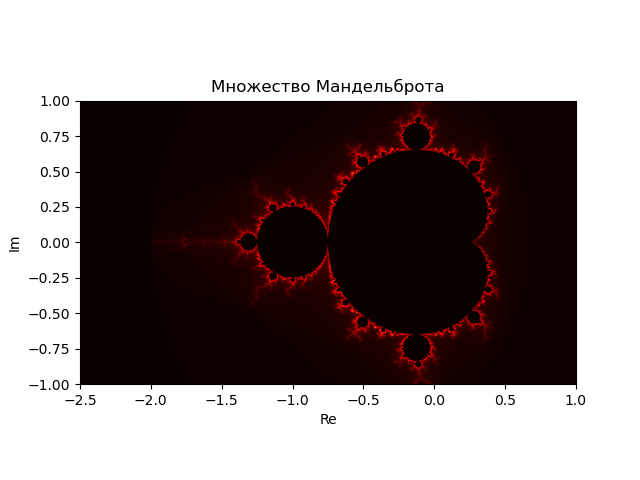
\includegraphics[width=1\textwidth]{images/screenshot001}
		\caption{Множество Мандельброта при максимальном числе итераций 100}
		\label{fig:mandelbrot}
	\end{figure}
	
	\newpage
	
	\section{Визуализация множества Жюлиа}
	
	\subsection{Описание алгоритма}
	Алгоритм для визуализации заполненного множества Жюлиа аналогичен алгоритму для множества Мандельброта, с той разницей, что параметр $c$ фиксирован, а начальные значения $z_0$ берутся из комплексной плоскости.
	
	\begin{enumerate}
		\item \textbf{Определение области комплексной плоскости:} Обычно выбирается квадратная область, например, $x, y \in [-1.5, 1.5]$.
		\item \textbf{Итерационный процесс:} Для каждого $z_0 = x + iy$ выполняем итерации:
		\begin{equation}
			z_{n+1} = z_n^2 + c,
		\end{equation}
		где $c$ — фиксированный параметр.
		\item \textbf{Определение цвета пикселя:} Аналогично множеству Мандельброта, определяем принадлежность точки множеству Жюлиа и окрашиваем пиксель.
	\end{enumerate}
	
	\subsection{Реализация на Python}
	
	\begin{lstlisting}[language=Python, inputencoding=utf8]
		import numpy as np
		import matplotlib.pyplot as plt
		
		# Parameters for the Julia set
		width, height = 800, 800
		max_iter = 200
		xmin, xmax = -1.5, 1.5
		ymin, ymax = -1.5, 1.5
		c = -0.5251993 + 0.5251993j  # Fixed parameter c
		
		# Create the complex plane
		x = np.linspace(xmin, xmax, width)
		y = np.linspace(ymin, ymax, height)
		X, Y = np.meshgrid(x, y)
		Z = X + 1j * Y
		
		# Initialize arrays
		M = np.full(Z.shape, True, dtype=bool)
		iterations = np.zeros(Z.shape, dtype=int)
		
		# Iterative process
		for i in range(max_iter):
			Z[M] = Z[M] ** 2 + c
			escaped = np.abs(Z) > 2
			iterations[M & escaped] = i
			M[M & escaped] = False
		
		# Visualization
		plt.figure(dpi=100)
		plt.imshow(iterations, extent=(xmin, xmax, ymin, ymax), cmap='twilight_shifted')
		plt.xlabel('Re')
		plt.ylabel('Im')
		plt.title(f'Filled Julia Set for c = {c}')
		plt.show()
	\end{lstlisting}
	
	\newpage
	
	\subsection{Результаты визуализации}
	% Здесь вставьте блок для изображения множества Жюлиа
	\begin{figure}[H]
		\centering
		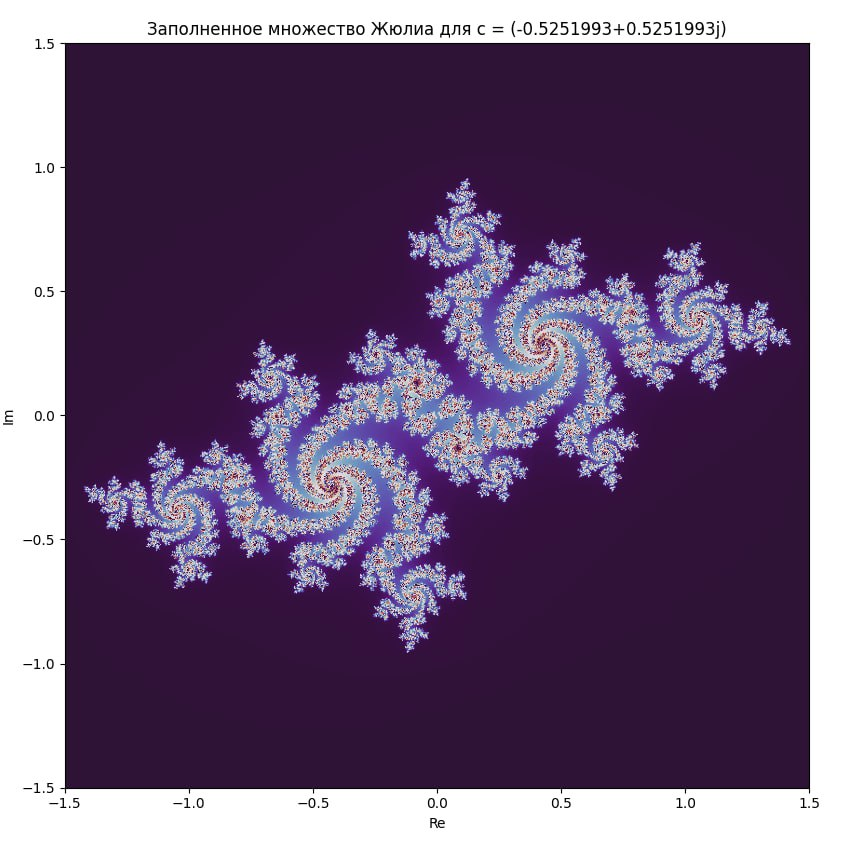
\includegraphics[width=0.8\linewidth]{images/screenshot002}
		\caption{Заполненное множество Жюлиа при $c = -0.5251993 + 0.5251993i$}
		\label{fig:julia}
	\end{figure}
	
	\newpage
	
	\section{Исследование другого фрактала: Фрактал Виксека}
	
	\subsection{Описание фрактала}
	Фрактал Виксека отличается своей простотой в построении и удивительной самоподобной структурой. Он создаётся путем рекурсивного деления квадрата на пять равных частей и удаления центральной части на каждом шаге итерации. В результате образуется структура, которая напоминает крест или плюс, обладающая интересными фрактальными свойствами.
	
	\subsection{Алгоритм построения}
	Основная идея построения фрактала Виксека заключается в рекурсивном делении квадрата на более мелкие части, что позволяет создать самоподобную и симметричную структуру.
	
	\textbf{Правила построения:}
	
	\begin{itemize}
		\item \textbf{Начало:} Начинаем с квадрата.
		\item \textbf{Итерация:} Делим текущий квадрат на 3 равных по длине отрезка по горизонтали и вертикали, образуя сетку из 9 меньших квадратов.
		\item \textbf{Удаление:} Удаляем средний квадрат, оставляя четыре угловых квадрата и центральный.
		\item \textbf{Повторение:} Повторяем тот же процесс для оставшихся квадратов на каждом уровне рекурсии.
	\end{itemize}
	
	\subsection{Реализация на Python}
	Ниже представлен пример кода на Python, который визуализирует фрактал Виксека с использованием библиотеки matplotlib и рекурсивной функции для построения фрактала.
	
\begin{lstlisting}[language=Python, inputencoding=utf8]
	import matplotlib.pyplot as plt
	import matplotlib.patches as patches
	
	def draw_vicsek(ax, x, y, size, level):
		if level == 0:
		# Draw the square
		square = patches.Rectangle((x, y), size, size, linewidth=1, edgecolor='black', 	facecolor='black')
		ax.add_patch(square)
		else:
		new_size = size / 3
		# Coordinates for the central and corner squares
		positions = [
		(x, y),  # bottom left
		(x + 2 * new_size, y),  # bottom right
		(x, y + 2 * new_size),  # top left
		(x + 2 * new_size, y + 2 * new_size),  # top right
		(x + new_size, y + new_size)  # center
		]
		for (nx, ny) in positions:
		draw_vicsek(ax, nx, ny, new_size, level - 1)
	
	def plot_vicsek(level):
		fig, ax = plt.subplots()
		ax.set_aspect('equal')
		ax.axis('off')
		
		# Initial coordinates and size
		x, y = 0, 0
		size = 1
	
		draw_vicsek(ax, x, y, size, level)
	
		plt.show()
	
	if __name__ == "__main__":
		# Recursion level (the higher, the more detailed)
		recursion_level = 4
		plot_vicsek(recursion_level)
	
\end{lstlisting}
	
	\subsection{Результаты визуализации}
	% Здесь вставьте блок для изображения фрактала Виксека
	\begin{figure}[H]
		\centering
		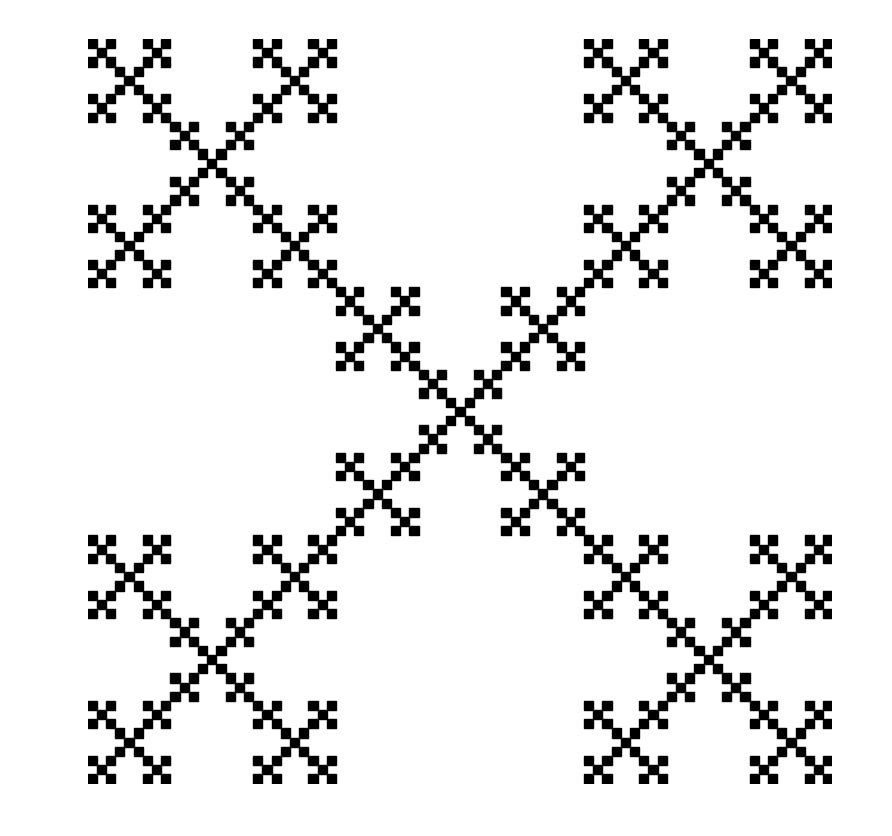
\includegraphics[width=0.8\textwidth]{images/screenshot_vicsek}
		\caption{Фрактал Виксека на уровне рекурсии 4}
		\label{fig}
	\end{figure}
	lab1
	\newpage
	
	\subsection{Анализ результатов}
	\textbf{Самоподобная структура:} Фрактал Виксека демонстрирует самоподобную структуру на каждом уровне рекурсии. С увеличением уровня детализации фрактал приобретает все более сложные и красивые геометрические узоры.
	
	\textbf{Симметрия и простота:} Основной особенностью фрактала Виксека является его симметрия и относительная простота построения. Даже при высоком уровне рекурсии структура остаётся легко узнаваемой, создавая уникальный геометрический рисунок, который можно наблюдать в различных масштабах.
	
	\newpage
	
	\section{Набор изображений при разных параметрах}
	
	\subsection{Множество Мандельброта при разных итерациях}
	% Здесь вставьте блоки для изображений множества Мандельброта при разных max\_iter
	\begin{figure}[H]
		\centering
		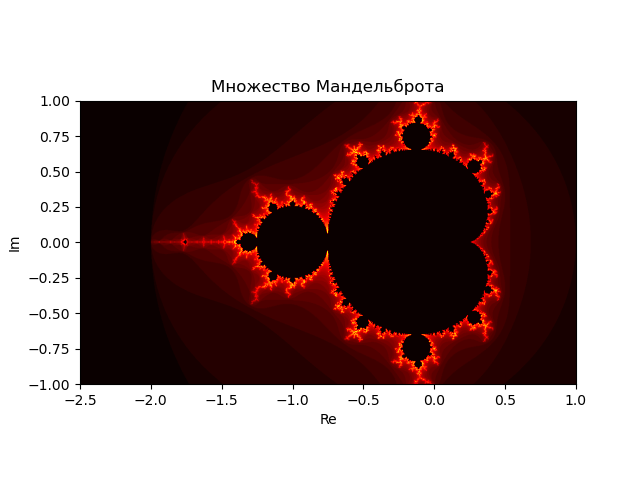
\includegraphics[width=0.8\textwidth]{images/mandelbrot_iter50.png}
		\caption{Множество Мандельброта при max\_iter = 50}
		\label{fig:mandelbrot50}
	\end{figure}
	
	\begin{figure}[H]
		\centering
		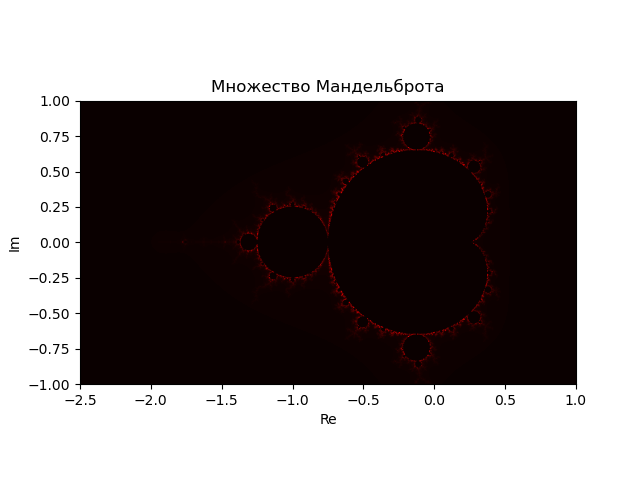
\includegraphics[width=0.8\textwidth]{images/mandelbrot_iter1000.png}
		\caption{Множество Мандельброта при max\_iter = 1000}
		\label{fig:mandelbrot1000}
	\end{figure}
	
	\subsection{Приближение отдельных частей множества Мандельброта}
	
	% Здесь вставьте блоки для приближённых изображений
	\begin{figure}[H]
		\centering
		% 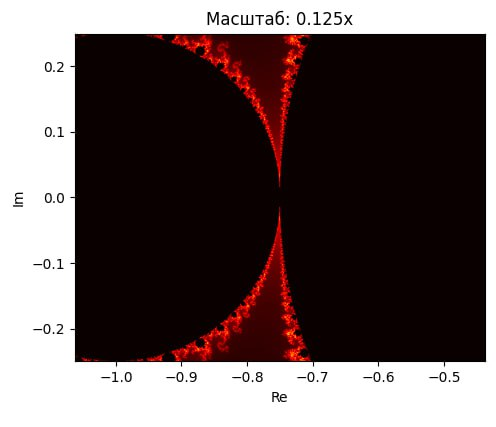
\includegraphics[width=0.8\textwidth]{mandelbrot_zoom1.png}
		\caption{Приближение области множества Мандельброта}
		\label{fig:mandelbrot_zoom1}
	\end{figure}
	
	\subsection{Множество Жюлиа при разных значениях $c$}
	% Здесь вставьте блоки для изображений множества Жюлиа при разных $c$
	\begin{figure}[H]
		\centering
		% 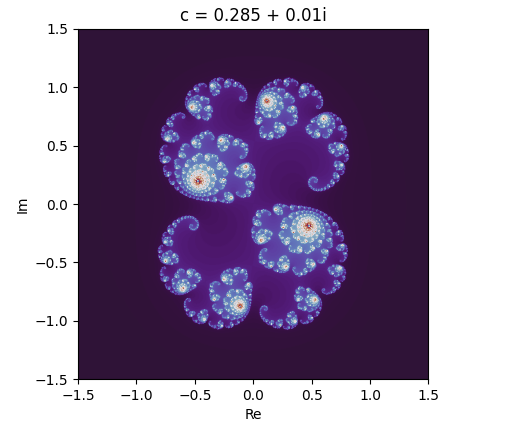
\includegraphics[width=0.8\textwidth]{julia_c1.png}
		\caption{Множество Жюлиа при $c = 0.285 + 0.01i$}
		\label{fig:julia_c1}
	\end{figure}
	
	\begin{figure}[H]
		\centering
		% 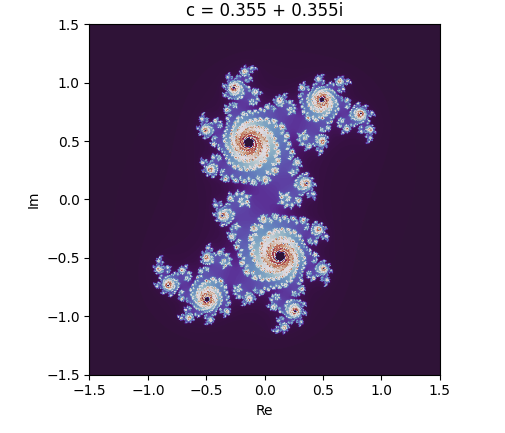
\includegraphics[width=0.8\textwidth]{julia_c2.png}
		\caption{Множество Жюлиа при $c = -0.70176 - 0.3842i$}
		\label{fig:julia_c2}
	\end{figure}
	
	\newpage
	
	\section{Заключение}
	В данной лабораторной работе мы подробно изучили множества Мандельброта и Жюлиа, доказали их основные свойства и реализовали алгоритмы для их визуализации. Мы также исследовали бассейны Ньютона, продемонстрировав фрактальную природу границ областей сходимости метода Ньютона к различным корням.
	
	Проведённые эксперименты показали, как простые итерационные процессы могут приводить к возникновению сложных и красивых фрактальных структур. Изменение параметров итераций и приближения позволило нам наблюдать разнообразие форм и узоров, присущих этим множествам.

	
\end{document}